\documentclass[main]{subfiles}

\begin{document}
    \newpage
    \subsection{Вычисление интеграла $\int_0^\infty \frac{\sin x}{x}dx$}

    \begin{Examples}
        \[\int_0^\infty \frac{\sin x}{x}dx = \frac{1}{2} (V.P.)\int_{-\infty}^{+\infty} \frac{\sin x}{x}dx  \]
        %рисунок1 ЛЖ
        \begin{figure}[H]
            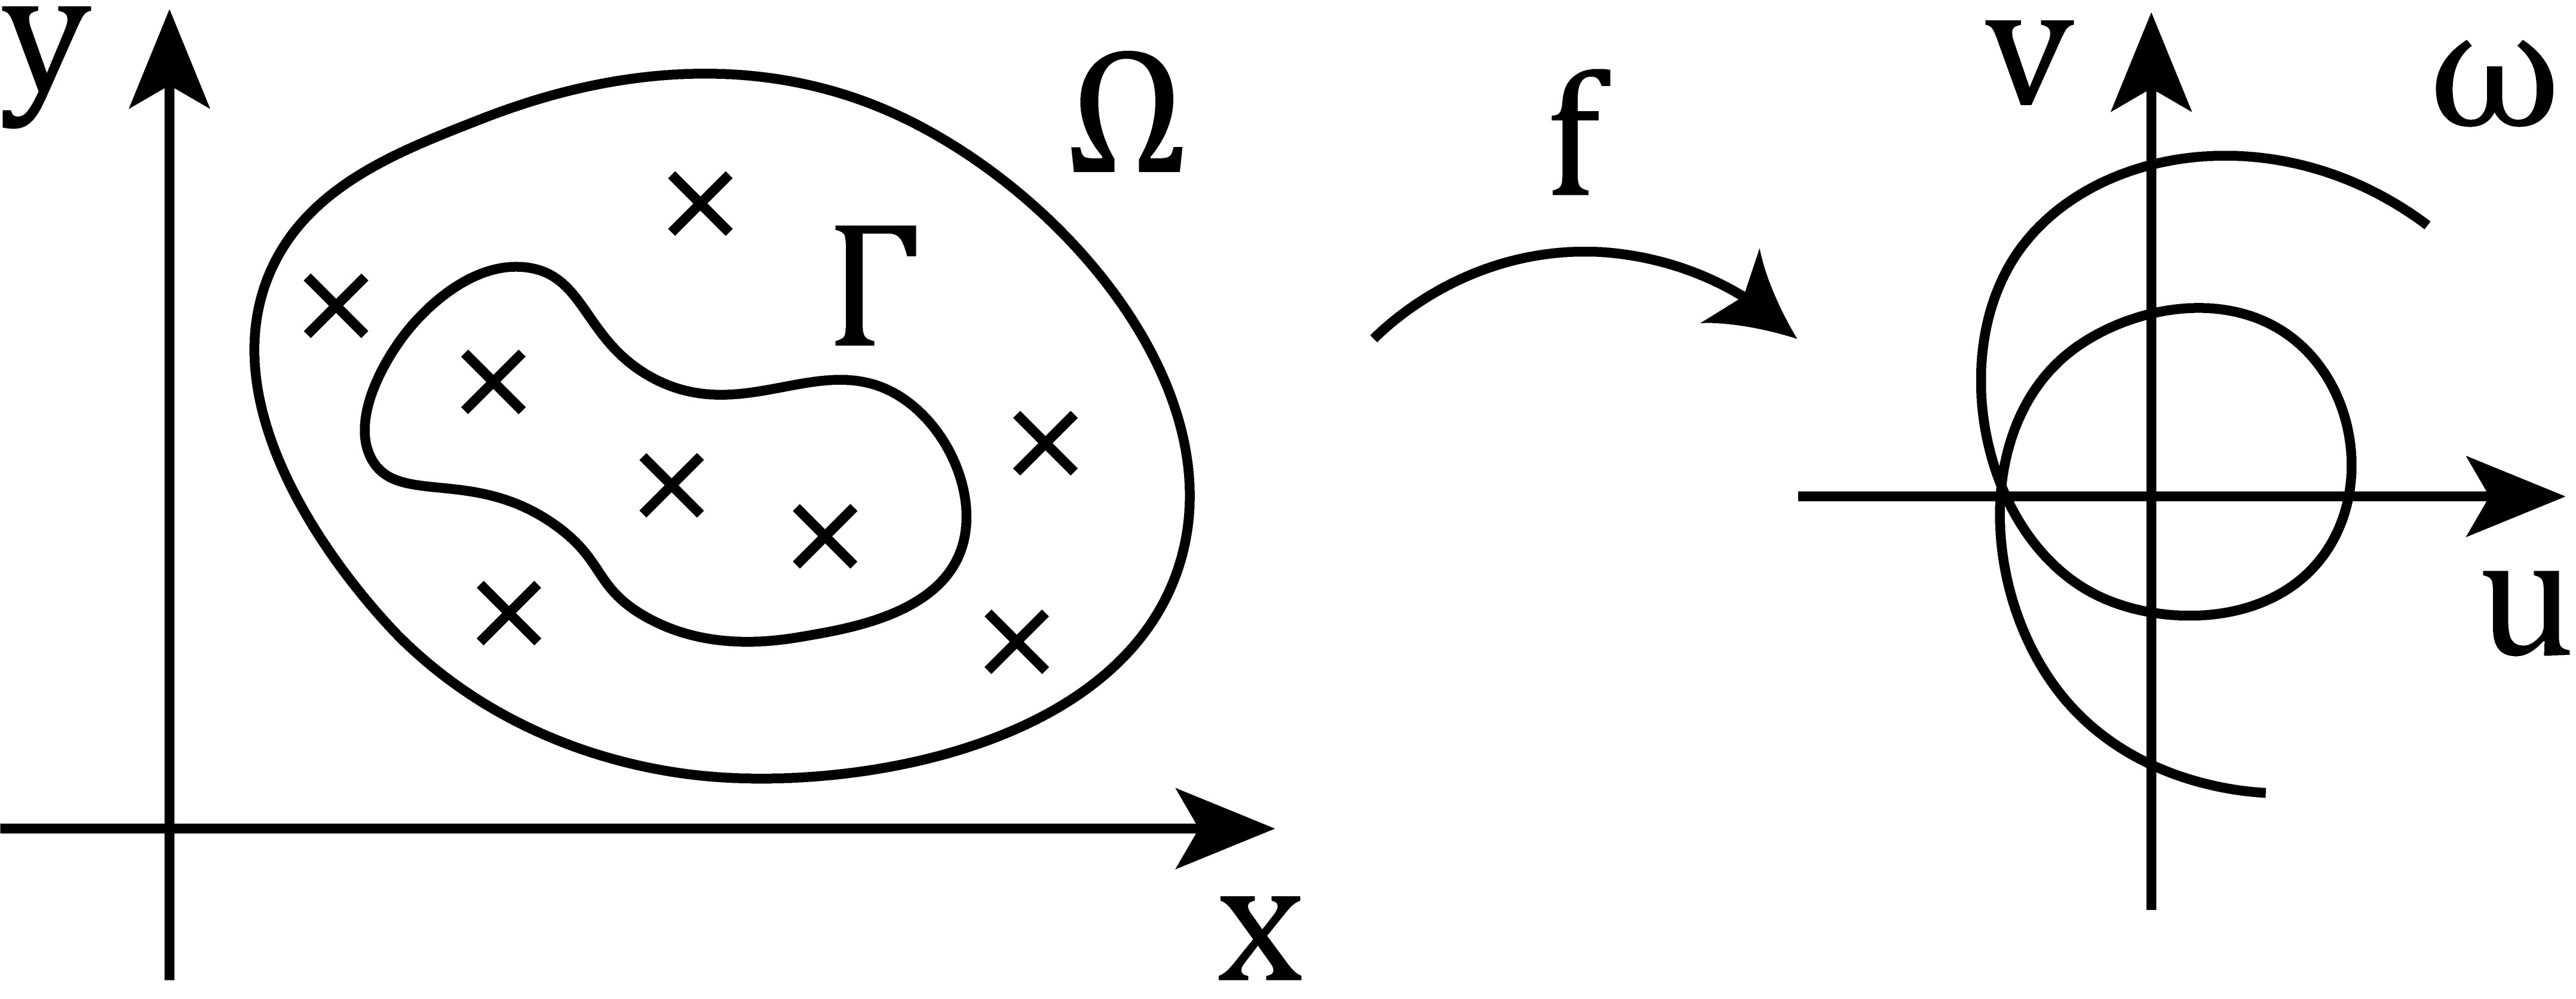
\includegraphics[width=7cm]{pics/14_1}
            \centering
        \end{figure}
        \[\int_0^A \frac{\sin x}{x}dx = \frac{1}{2} \int_A^A \frac{\sin x}{x}dx\]
        \[f \in C(z : \abs{z} \geq R, \Im z > 0)\]
        \[M_\rho = \max_{0 \leq t \leq \pi } \]
        Дописать %я опоздал
        \[(V.P.) \int_{-\infty}^{+\infty} \frac{x}{x^2 + \mathcal{E}^2} \sin x dx =
            \lim_{A \to +\infty}  \int_{-A}^{A}  \]
        %пропуск
        \[\text{по т. о выч. } \int_{\Gamma_A} \frac{z}{z^2 + \mathcal{E}^2}e^{iz}dz =
            2\pi i \res_{\mathcal{E}i} \frac{z}{z^2 + \mathcal{E}^2} e^{iz} =   \]
        \[= 2\pi i \lim_{z \to i\mathcal{E}} \frac{ze^{iz} }{z + i\mathcal{E}} = 2\pi i
            \frac{i\pi e^{-\mathcal{E}} }{2i\mathcal{E}} = \pi i e^{-\mathcal{E}} \]
        \[\text{по л. Ж } \int_{C_A} \frac{z}{z^2 + \mathcal{E}^2}e^{iz}dz \us{A \to +\infty}{\to } 0  \]
        \[\int_{-\infty}^{+\infty} \frac{ze^{iz}dz }{z^2 + \mathcal{E}^2} =
            [z = x + i\cdot 0] = \int_{-\infty}^{+\infty} \frac{x(\cos x + i\sin x)}{x^2 + \mathcal{E}^2}dx =  \]
        \[ = \pi i e^{-\mathcal{E}} \]
        \[\int_{-\infty}^{+\infty} \frac{x\sin x}{x^2 + \mathcal{E}^2}dx = \Im (\pi ie^{-\mathcal{E}} ) =
            \pi e^{-\mathcal{E}} \us{??}{\to } \pi \]%дописать
    \end{Examples}

    \newpage
    \subsection{Логарифмический вычет}

    \begin{Definition}
        \[F \in H(\Omega \setminus \{z_1, ..., z_n\}) \qq \Gamma \subset \Omega \setminus \{z_1, ..., z_n\}\]
        \[f \bigg|_\Gamma \neq 0\]
        %рисунок2
        \begin{figure}[H]
            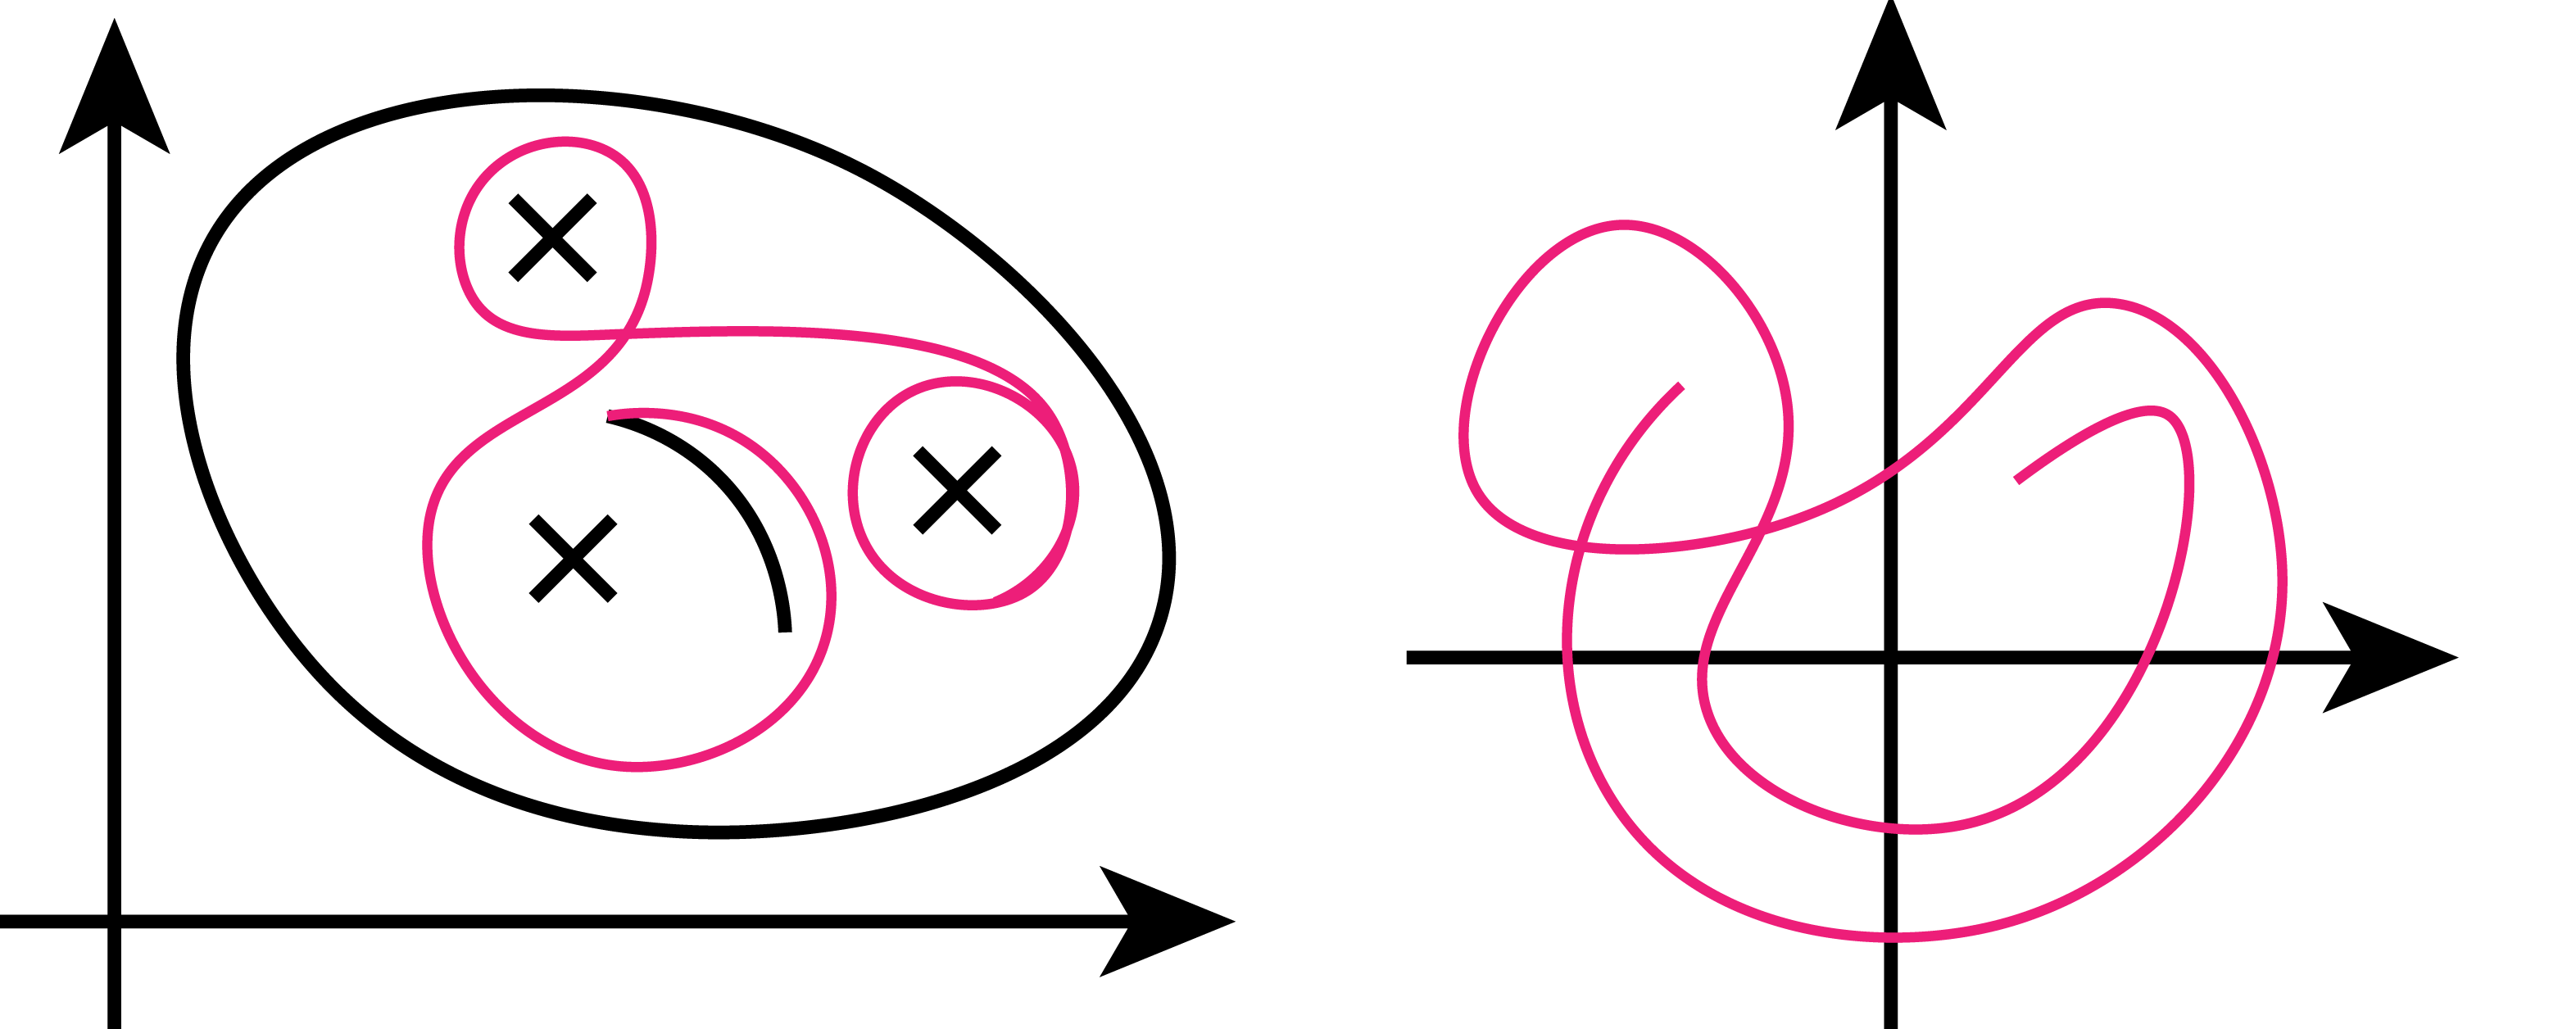
\includegraphics[width=6cm]{pics/14_2}
            \centering
        \end{figure}

        Образ кривой
        \[f(\Gamma) = \widetilde{\Gamma} \text{ --- кривая, причем } 0 \not \in \widetilde{\Gamma}\]
        %рисунок2
        Рассмотрим
        \[\Ln f(z) \text{ на } \Gamma\]
        \[\Ln f(z) = \us{\text{однознач. ф-я}}{\ln \abs{f(z)}} + \us{\text{многознач. ф-я}}{i\Arg f(z)}\]
        \[(\Ln f(z))' = \frac{f'(z)}{f(z)}\]
        \[z_2 \text{ --- конец пути } \qq z_1 \text{ --- начало пути}\]
        \[\int_\Gamma \frac{f'(z)}{f(z)}dz = \int_\Gamma (\Ln f(z))'dz \us{\text{по ф-ле Н-Л}}{= }
            \Ln f(z_2) - \Ln f(z_1) = \Delta_\Gamma \Ln f(z)\]
        %рисунок 3
        \begin{figure}[H]
            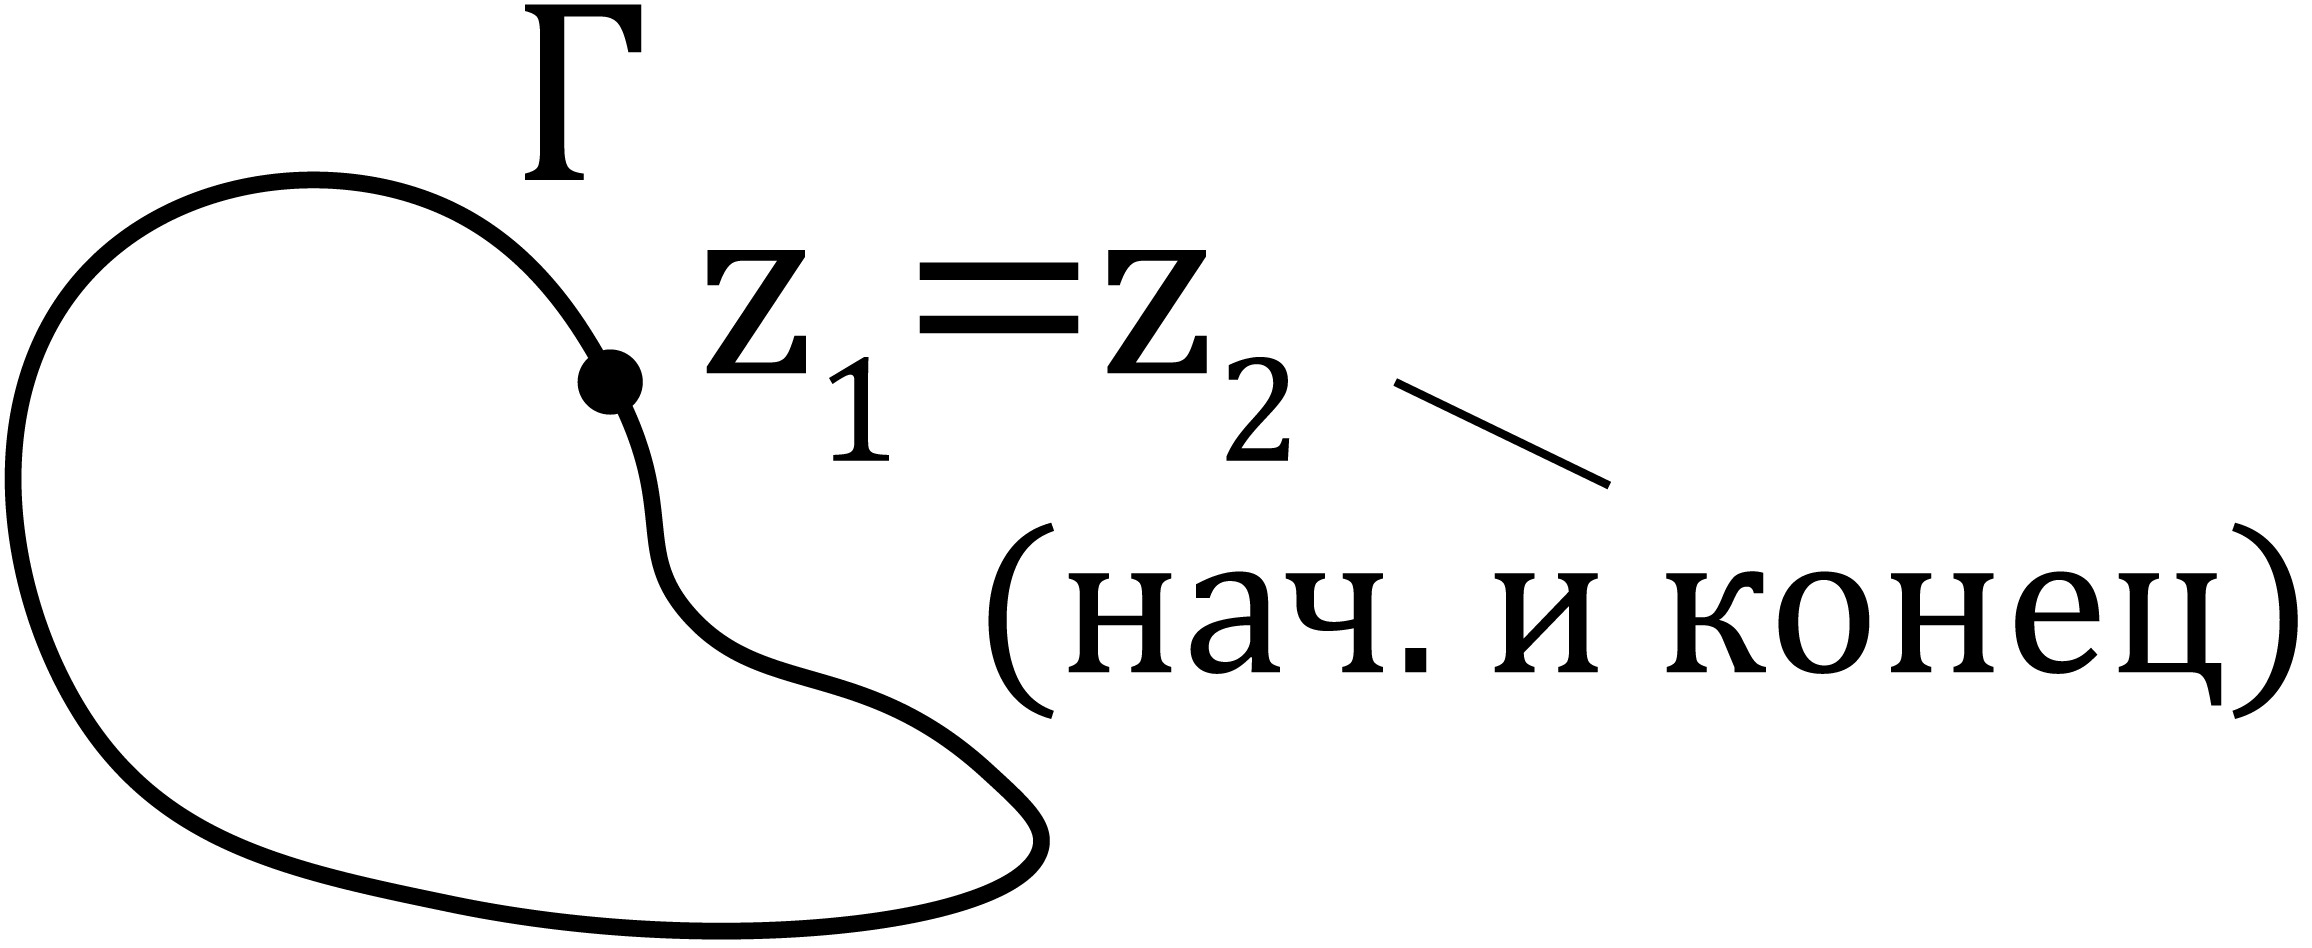
\includegraphics[width=5cm]{pics/14_3}
            \centering
        \end{figure}
        --- изменение лог-ма $f(z)$ после обх. вдоль $\Gamma$\\
        После обхода $z$ вдоль $\Gamma$ ($f(z)$ --- вдоль  $\widetilde{\Gamma}$)
        при возвр. в начало пути $\arg f(z)$ может отличаться от начального знач. на
        $2\pi k, \q k \in \Z$
        \[\text{А т.к. } \Ln f(z) = \us{\text{не изм}}{ \ln \abs{f(z)}} +
            i\us{\text{изм на } 2\pi k}{\Arg f(z)}\ \Ra\  \Delta_\Gamma
            \Ln f(z) = 2\pi k i, \q k \in \Z\]
        \[\text{т.о } \int_{\Gamma} \frac{f'(z)}{f(z)}dz = 2\pi k i, \q k \in \Z \]
    \end{Definition}

    \begin{definition}
        Пусть $f$ --- мероморфная (т.е. все её особые т. --- полюса) в $\Omega$
        \[f \in H(\Omega \setminus \{\us{\text{полюсы } f}{a_1, ..., a_p}\})\]
        Нули $f$ : $\{b_1, ..., b_N\} \subset \Omega$
        (пишем нули и полюса с учетом кратности, т.е. $a_i$ и $a_j$ могут совпадать)
        %рисунок4
        \begin{figure}[H]
            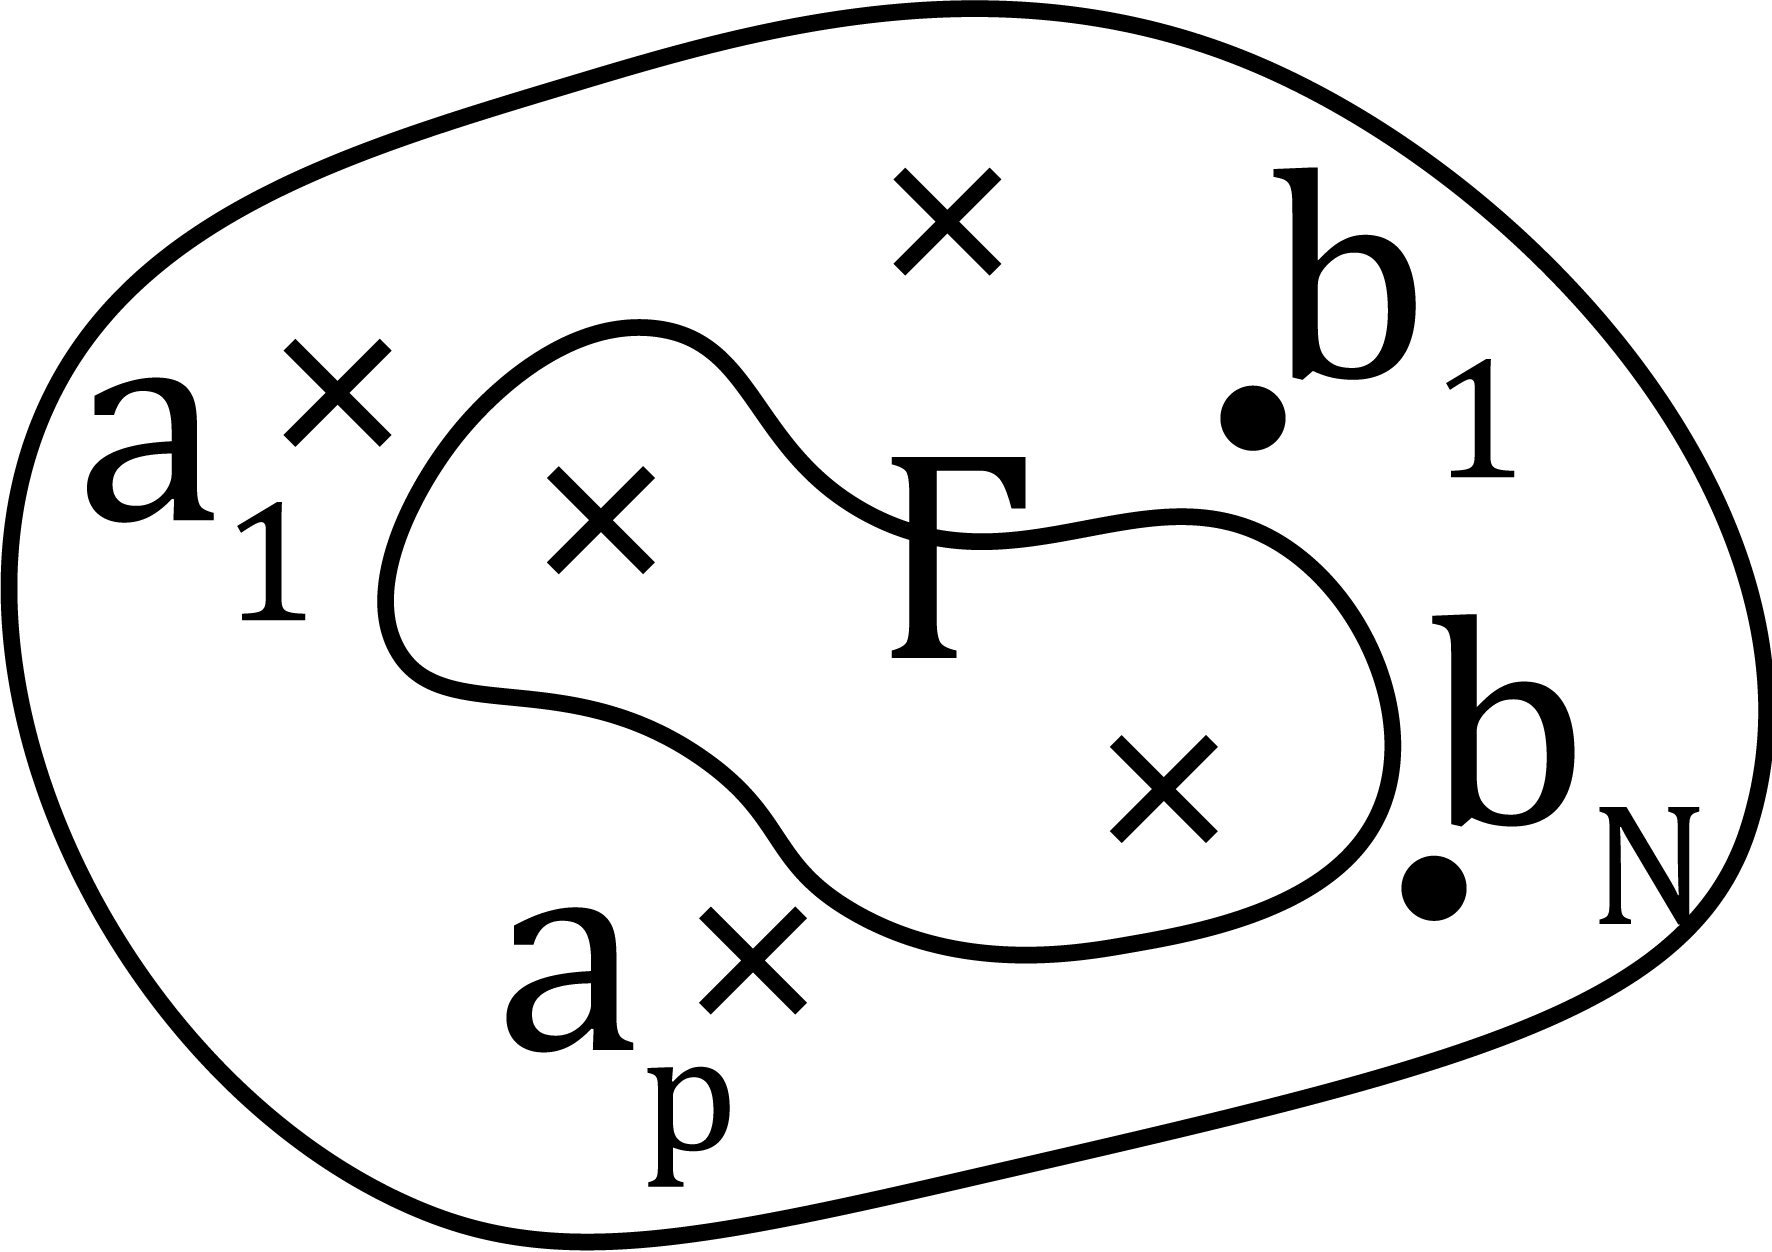
\includegraphics[width=3.5cm]{pics/14_4}
            \centering
        \end{figure}
        \[\us{\text{простой }}{\Gamma} \subset \Omega \setminus \{a_1,..., a_p, b_1, ..., b_N\}\]
        \[N^*, P^* \text{ --- кол-во нулей и полюсов внутри  } \Gamma (\text{с учетом кратности})\]
        Если $b_k$ - ноль $f$ кратности $q$
        \[f(z) = (z - b_k)^q \varphi(z)\q \text{ причем } \varphi \text{ - аналит, } \varphi(b_k) \neq 0\]
        \[\frac{f'(z)}{f(z)} = \frac{q(z - b_k)^{q - 1} \varphi(z) + (z - b_k)^q \varphi'(z) }
            {(z - b_k)^q \varphi(z)} = \frac{q}{z - b_k} +
            \us{\us{= \text{ряд Тейлора}}{\text{аналит. в окр. }b_k}}{\frac{\varphi'(z)}{\varphi(z)}}\]
        \[\res_{b_k} \frac{f'(z)}{f(z)} = q; \q \text{ если } b_k \text{ - ноль кратности } q \ \  f \Ra  \]
        \[\Ra b_k \text{ --- полюс порядка } 1 \ \ \frac{f'}{f} \text{, причем }
            \res_{b_k} \frac{f'}{f} = q \]
        Если $a_k$ --- полюс порядка $r$
        \[f(z) = (z - a_k)^r g(z) \qq g(z) \text{ аналит. в окр. } a_k \qq g(a_k) \neq 0\]
        \[\frac{f'(z)}{f(z)} = \frac{r(z - a_k)^{-r - 1}g(z) + (z - a_k)^{-r}g^'(z) }{(z - a_k)^{-r}
                g(z)} = \frac{-r}{z - a_k} + \frac{g'(z)}{g(z)}\]
        \[\Ra a_k \text{ - полюс } \frac{f'(z)}{f(z)} \text{ порядка 1, причем }\]
        \[\res_{a_k} \frac{f'(z)}{f(z)} = -r \]
    \end{definition}

    \newpage
    \subsection{Принцип аргумента}

    \begin{Theorem}[принцип аргумента]\
        %рисунок5
        \begin{figure}[H]
            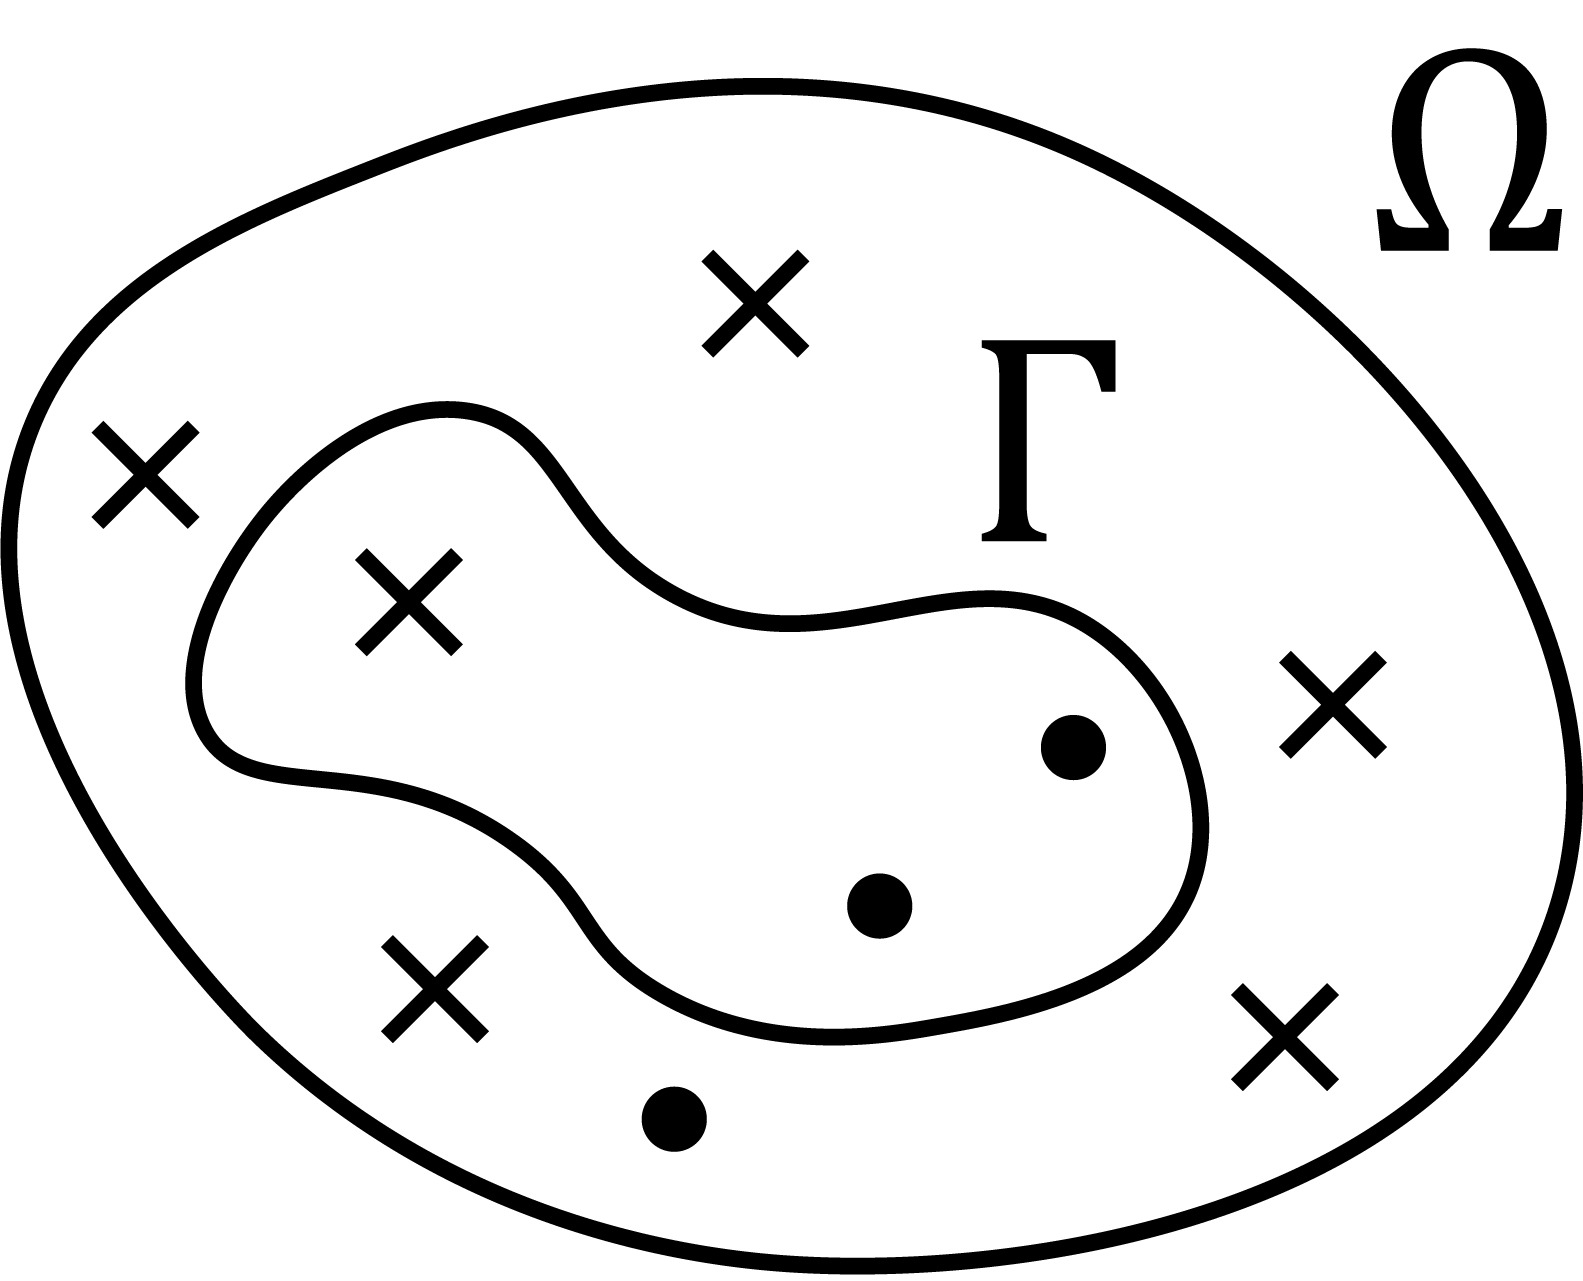
\includegraphics[width=3cm]{pics/14_5}
            \centering
        \end{figure}
        \[f \us{\text{в } \Omega}{\text{ --- мером.}}\]
        \[\frac{1}{2\pi}\Delta_\Gamma \arg(f(z)) = N^* - P^*\]
        \[\text{где }N^*, P^* \text{ --- число нулей и полюсов с учетом кратности внутри } \Gamma\]
    \end{Theorem}

    \newpage
    \subsection{Теорема Руше. Пример}

    \begin{Theorem}[Руше]
        \[\text{Пусть }\Omega; \q f, g \in H(\Omega); \q \Gamma \subset \Omega\]
        \[\forall z \in \Gamma \qq \abs{f(z)} > \abs{g(z)} \geq 0\]
        \[\text{Тогда } f \text{ и } f + g \text{ имеет внутри  } \Gamma \text{ одинаковое количество нулей}\]
        с учетом кратности
    \end{Theorem}

    \begin{Proof}
        \[Z_{f + g} \text{ --- кол-во нулей } f + g \text{ внутри } \Gamma\]
        \[Z_f \text{ --- кол-во нулей } f \text{ внутри } \Gamma\]
        \[Z_{f + g} = \frac{1}{2\pi} \Delta_{\Gamma}  \arg (\us{f(z)(1 + \frac{g(z)}{f(z)})}{f(z) + g(z)}) \]
        \[f(z) \neq 0 \text{ на } \Gamma \qq (\text{ т.к. }  \abs{f(z)} > \abs{g(z)} \geq 0 \q \forall z
            \in \Gamma)\]
        %рисунок6
        \begin{figure}[H]
            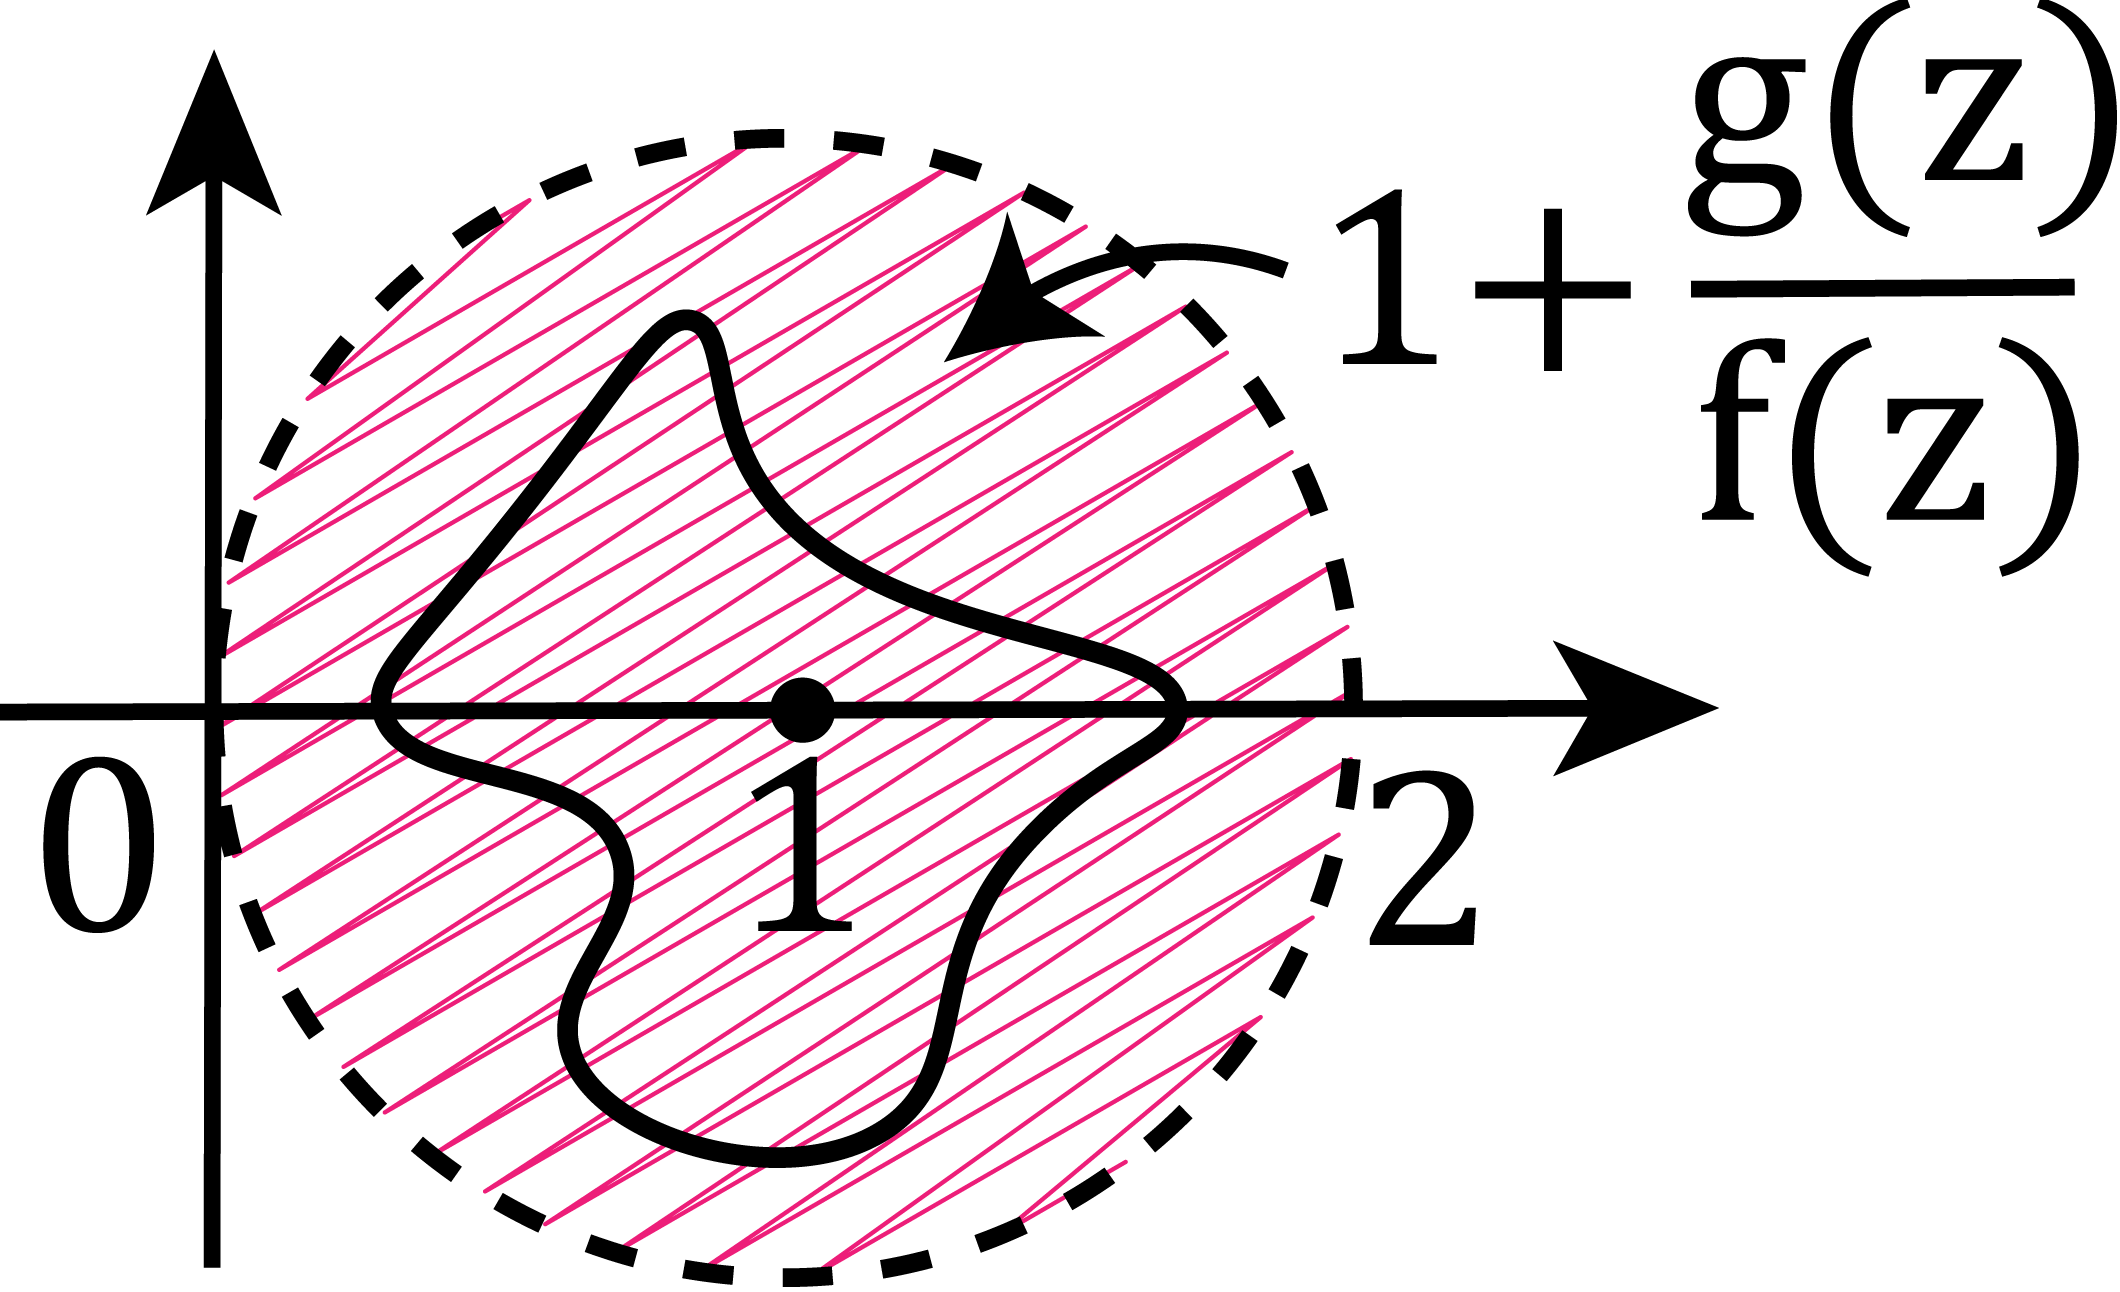
\includegraphics[width=3.7cm]{pics/14_6}
            \centering
        \end{figure}
        \[\abs{\frac{g(z)}{f(z)}}_\Gamma < 1\]
        \begin{multline*}
            \left(1 + \frac{g(z)}{f(z)}\right) \text{ при обходе вдоль }  \Gamma \q \text{ не совершает}\\
            \text{ ни одного оборота вокруг 0}
        \end{multline*}
        \[2\pi Z_{f + g} = \Delta_\Gamma \arg(f(z)(1 + \frac{g(z)}{f(z)})) =
            \Delta_\Gamma \arg f(z) + \us{= 0 }{\Delta_\Gamma \arg \left(1 + \frac{g(z)}{f(z)}\right)} = \]
        \[=\Delta_\Gamma \arg f(z) = 2\pi Z_f\]
    \end{Proof}

    \begin{Example}
        \[P(z) = z^7 + 4z^4 + z^3 + 1\]
        \begin{enumerate}
            \item $\Gamma : \q \abs{z} = 1$
                  \[f(z) = 4z^4 \qq g(z) = z^3 + z^3 + 1\]
                  \[\abs{f(z)} = 4 \text{ на } \Gamma : \abs{z} = 1\]
                  \[\abs{g(z)} = \abs{z^7 + z^3 + 1} \leq 3 < \abs{f(z)}\]
                  По т. Руше
                  \[Z_f = Z_P = 4\]
            \item $\Gamma : \ \abs{z} = 2$
                  \[f(z) = z^7 \qq \abs{f(z)}_\Gamma = 128\]
                  \[\abs{g(z)} = \abs{4z^4 + z^3 + 1} \leq 64 + 8 + 1 < 128 \]
                  \[\text{т.о. внутри  }\abs{z} = 2  \q 7 \text{ нулей}\]
        \end{enumerate}
    \end{Example}

    \newpage
    \subsection{Гармонические функции, связь с аналитическими}

    \begin{Definition}
        \[u(x, y) \text{ --- гармонич. в } \Omega \subset \R^2 \ \rla\ u \in C^2(\Omega) \text{ и } \]
        \[\Delta u = \frac{\d^2 u}{\d x^2} + \frac{\d^2 u}{\d y^2} = 0 \qq \text{ в } \Omega\]
    \end{Definition}

    \begin{Utv}
        \[\text{Если } \us{\text{однозн.}}{f} \in H(\Omega) \Ra u(x, y) =
            \Re f(z) \text{ --- гармонич. } \q (z = x + iy)\]
        А наоборот?\\
        Если $u$ --- гармонич. в $\Omega$ $\us{?}{\Ra} \ \exists f \in H(\Omega): \ \Re f = u ?$
        (Нет)
    \end{Utv}

    \begin{Example}
        \[u(x, y) = \frac{1}{2} \ln(x^2 + y^2) \qq \Omega \{(x, y) : \ 1 < x^2 + y^2 < 2\}\]
        %рисунок7
        \begin{figure}[H]
            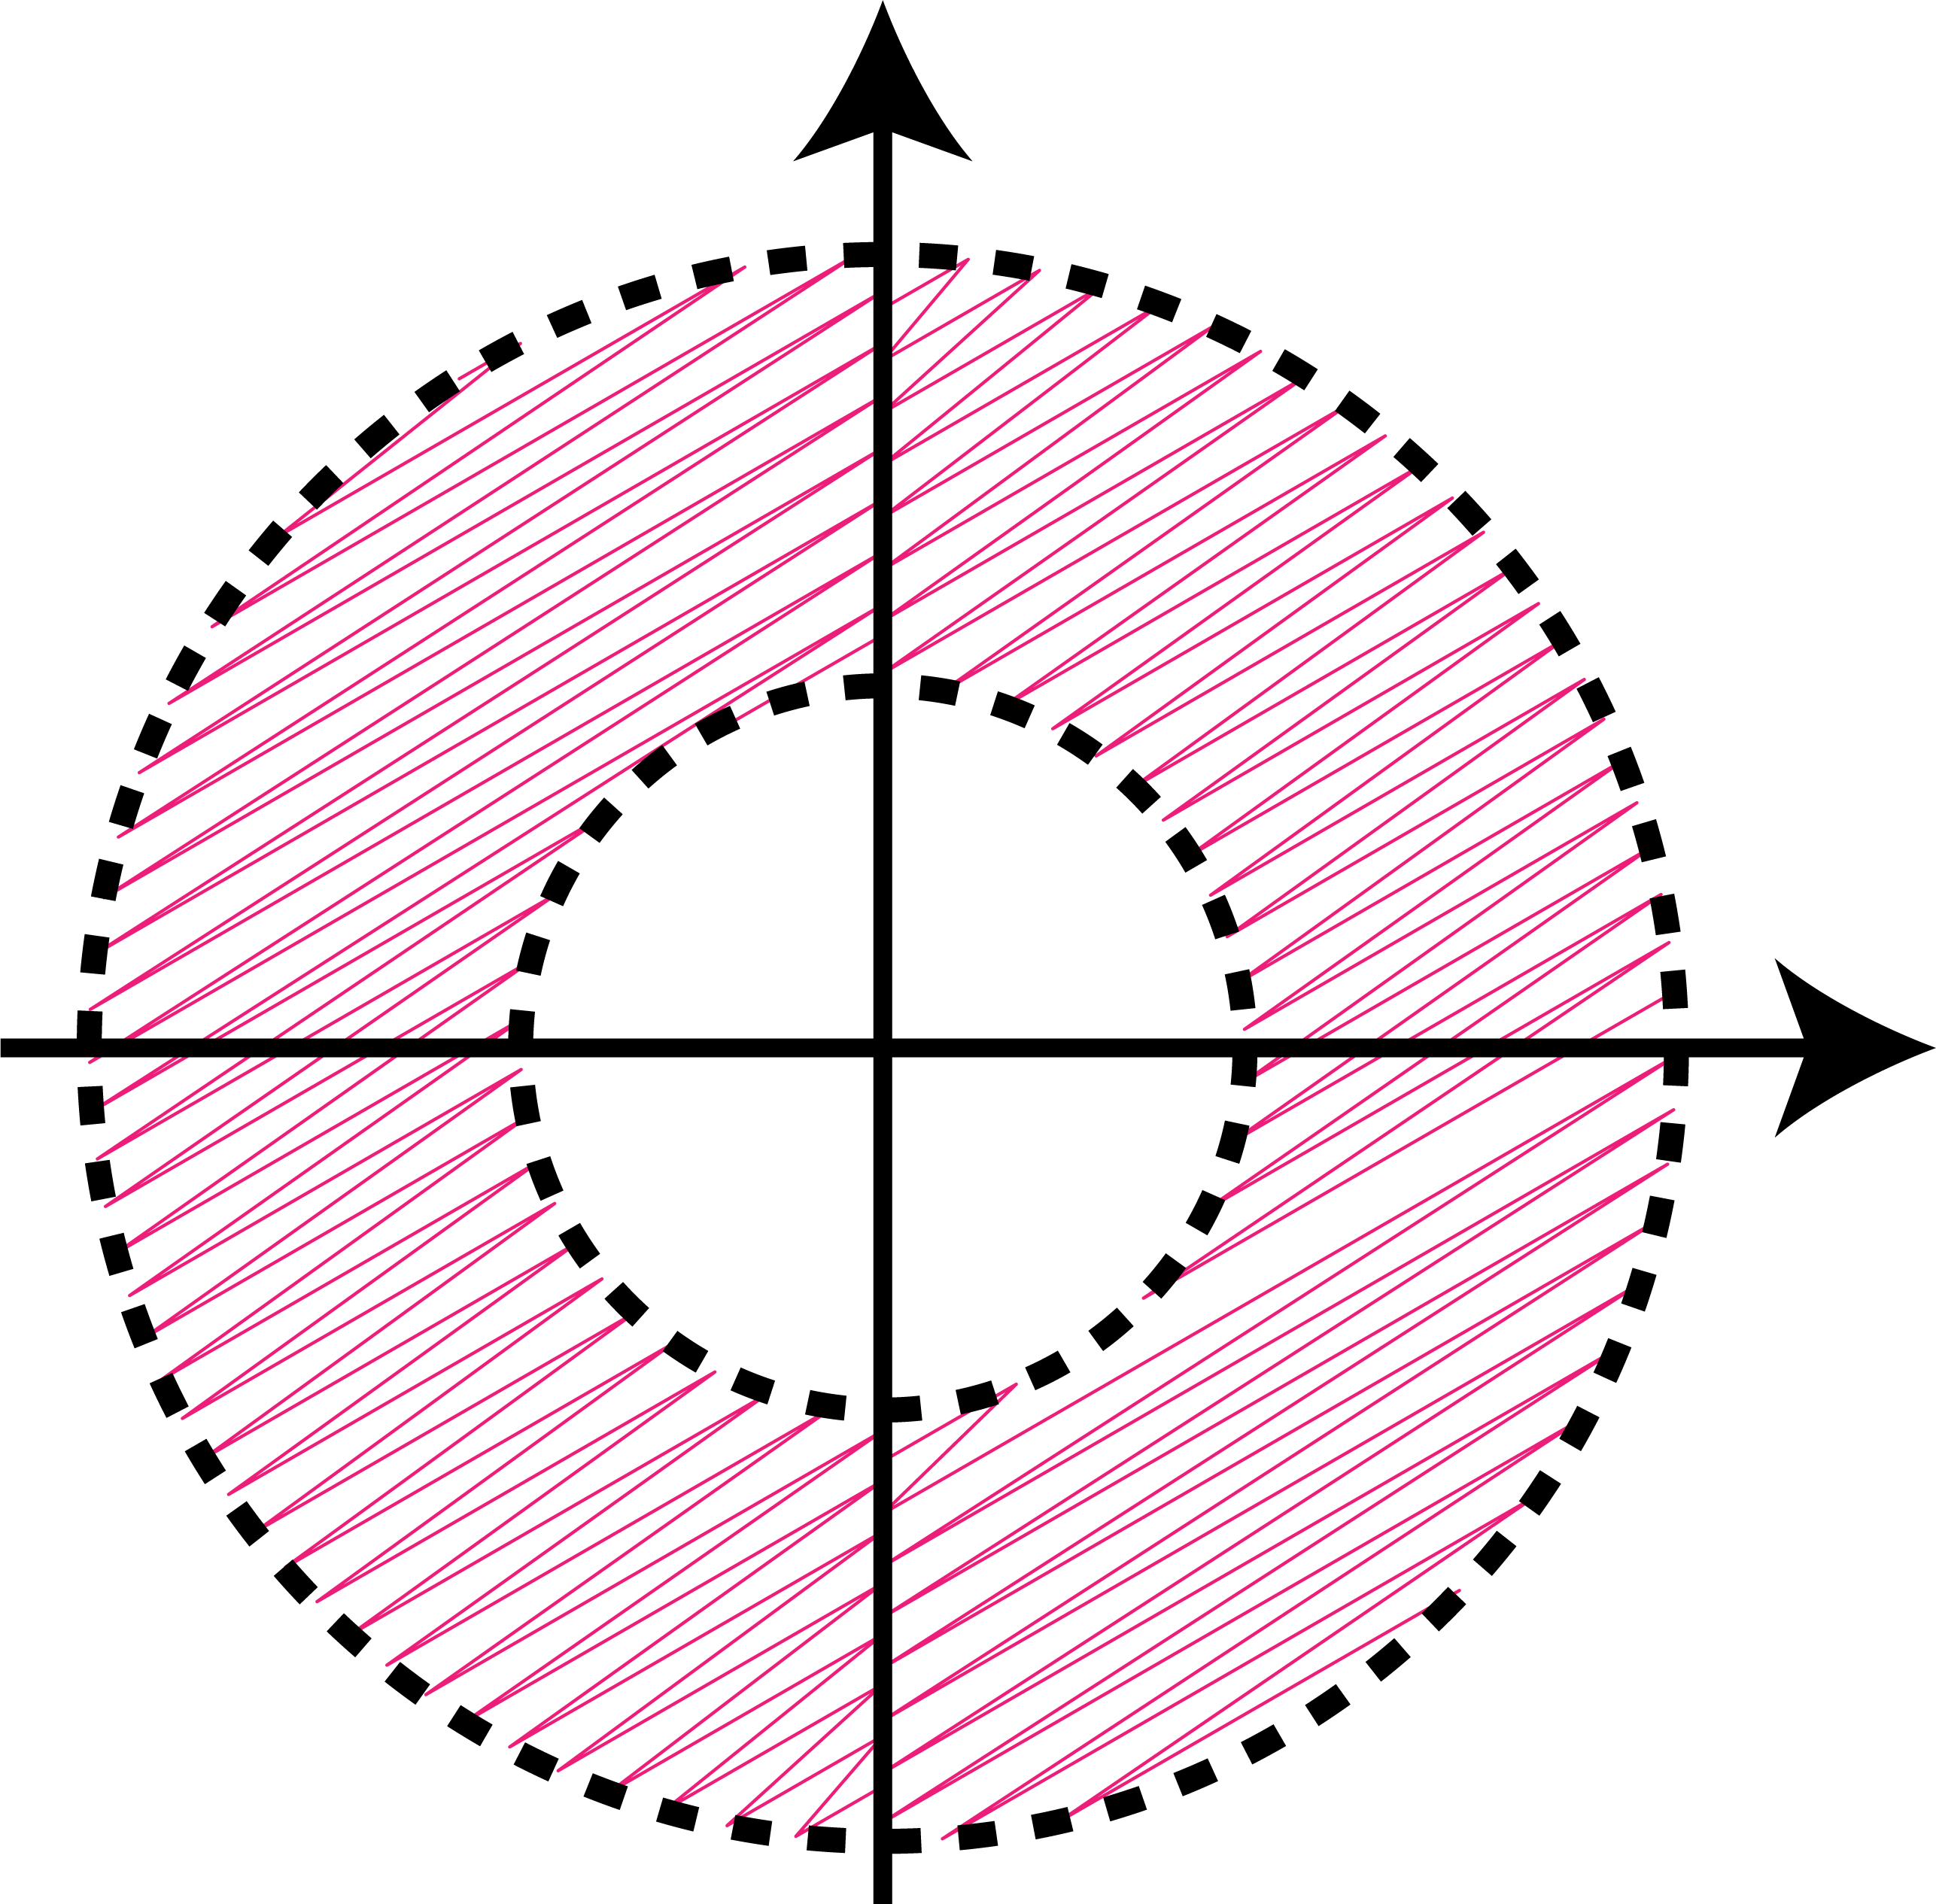
\includegraphics[width=3cm]{pics/14_7}
            \centering
        \end{figure}
        \[u \in C^\infty(\Omega)\]
        \[\Delta u = \frac{\d^2 u}{\d x^2}  +\frac{\d ^2 u}{\d y^2}\]
        \[u'_x = \frac{x}{x^2 + y^2}  \qq u''_{xx} = \frac{y^2 - x^2}{(x^2 + y^2)^2} \q
            u''_{yy} = \frac{x^2 - y^2}{(x^2 + y^2)^2} \]

        \[? \exists ? f \in H(\Omega) \qq \Re f = \frac{1}{2}\Ln(x^2 + y^2) ? \]
        \[f(z) = \Ln(z) = \ln \abs{z} + i\arg z = \underbracket{\frac{1}{2}\ln(x^2+ y^2)}_u +
            i\arg z\]
        Но $\Ln z \not \in H(\Omega)$ т.к. многознач.
        \[\widetilde{\Omega} = \Omega \cap \{\Im z > 0\}\]
        \[f \in H(\widetilde{\Omega})\]
        \[\Re f = u\]
        %рисунок 8
        \begin{figure}[H]
            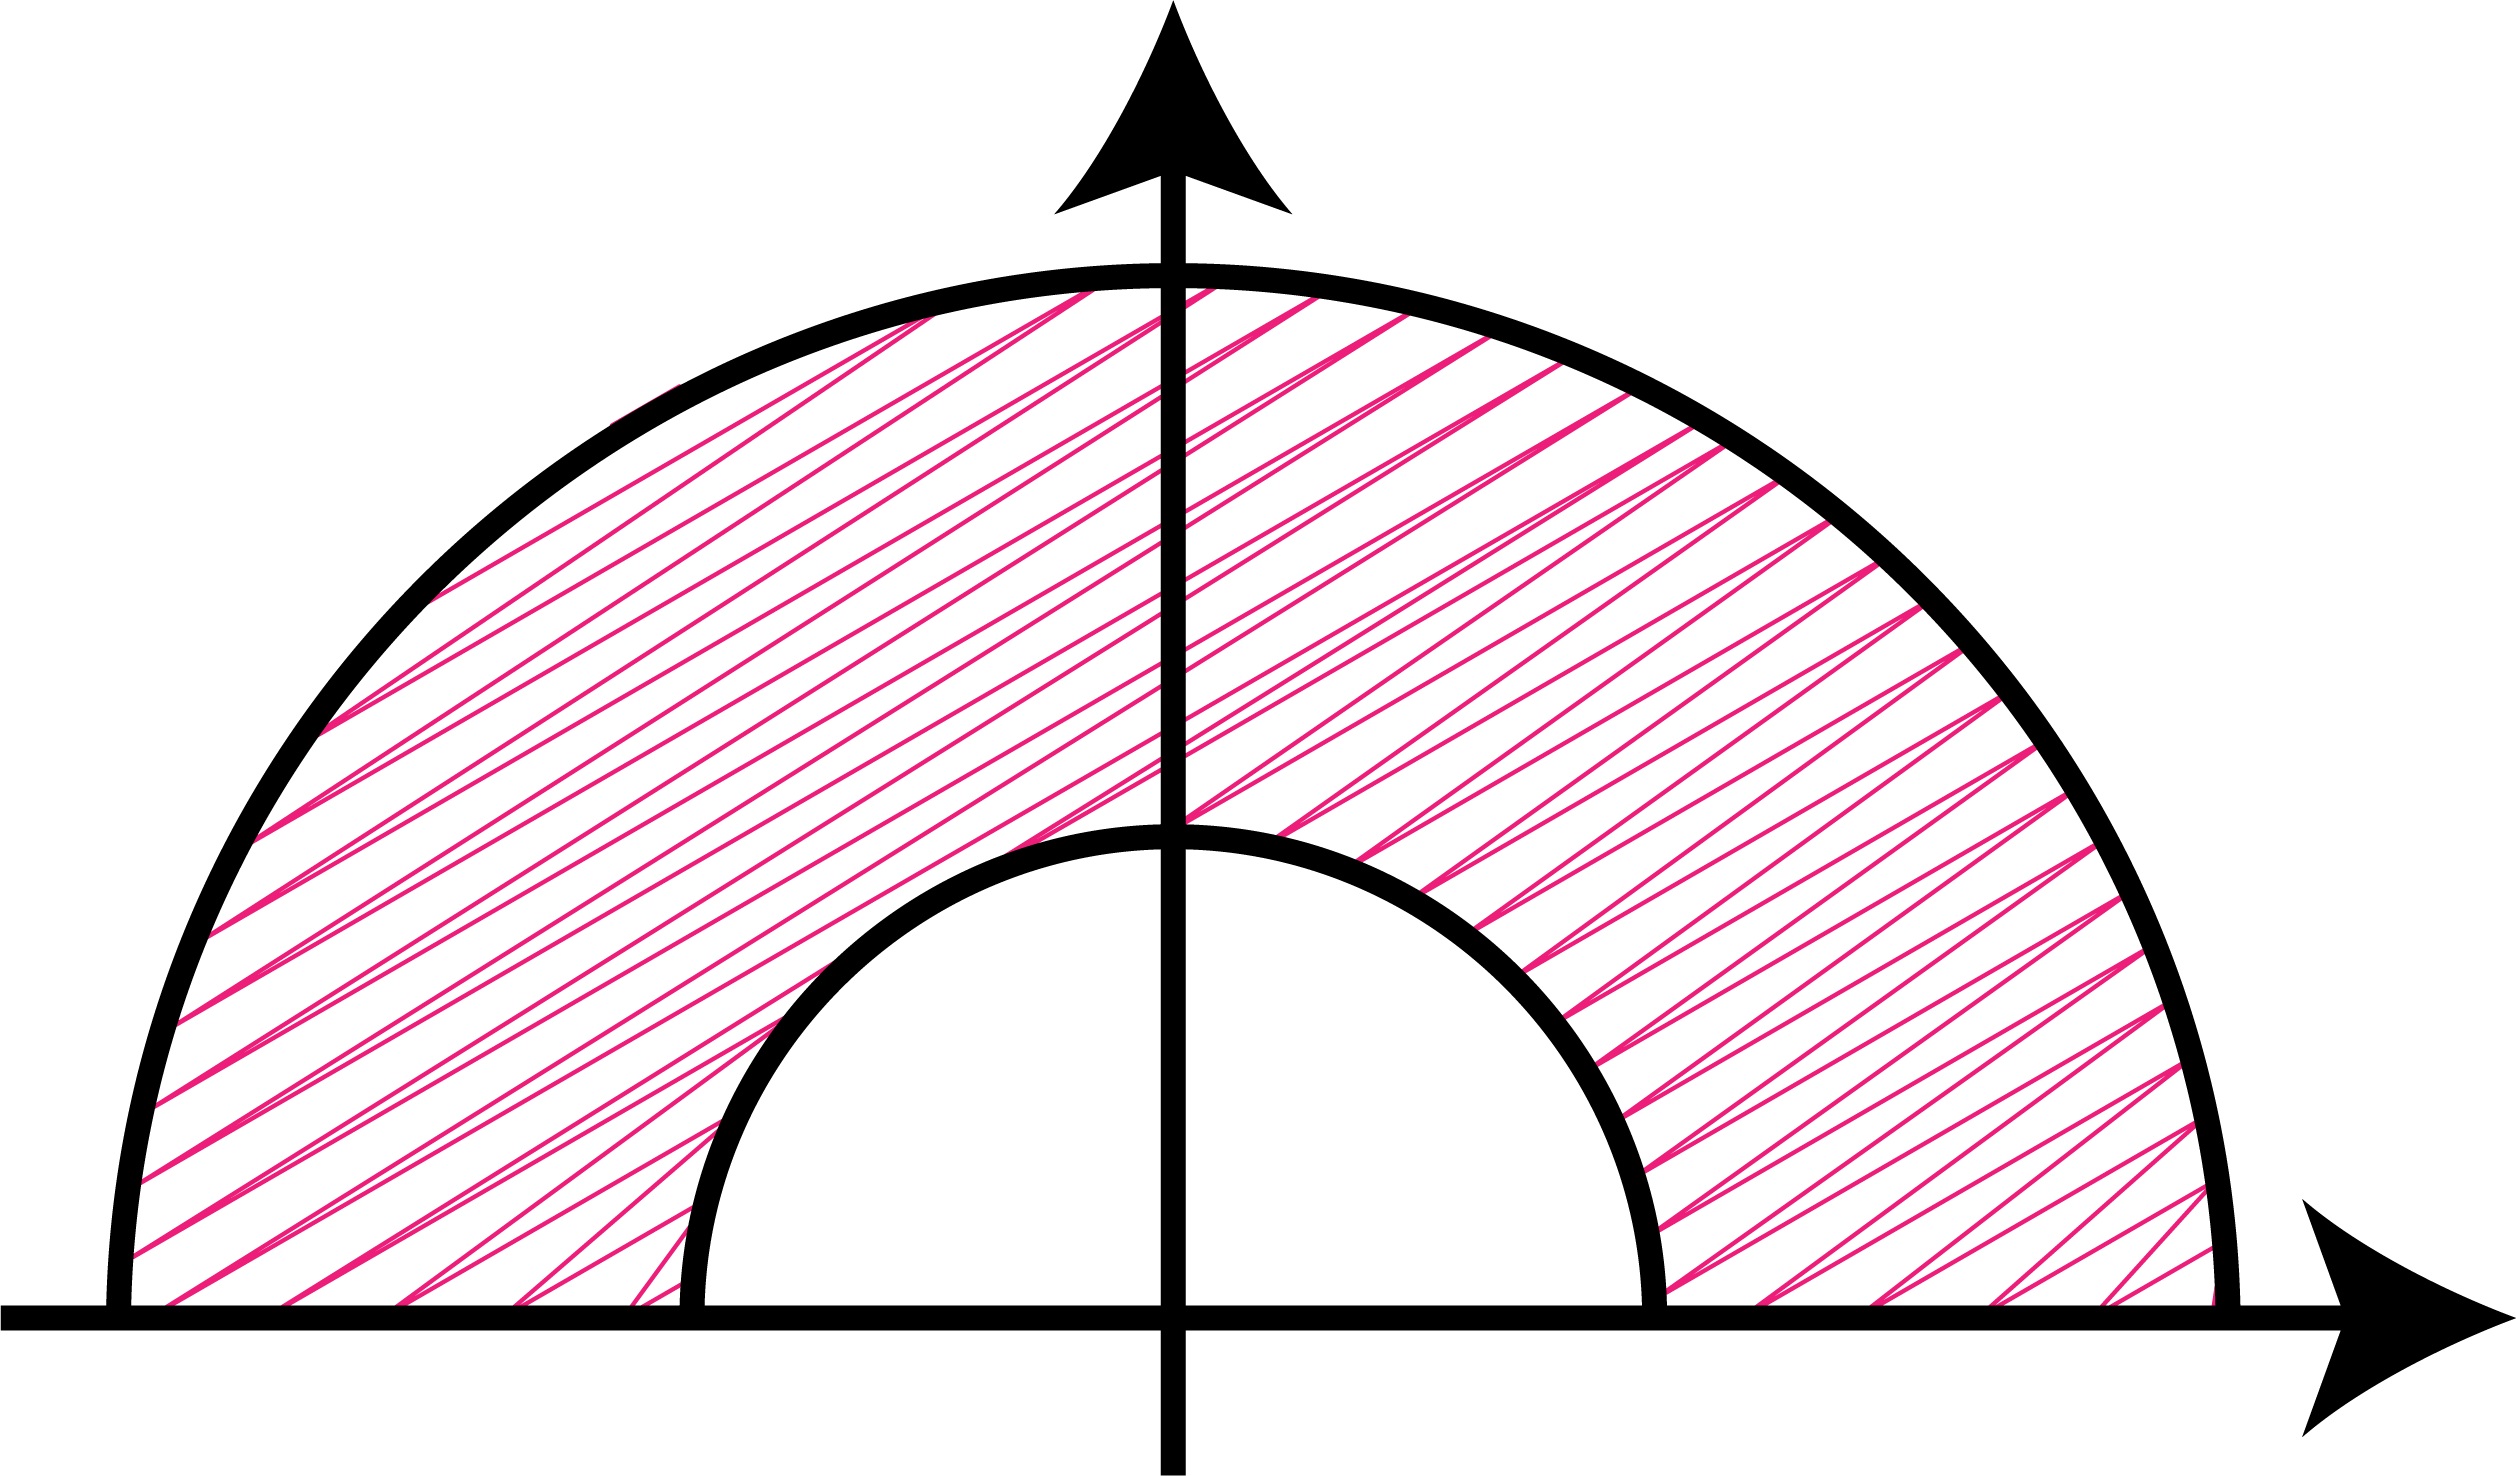
\includegraphics[width=3cm]{pics/14_8}
            \centering
        \end{figure}
        То есть,  в общем случае ответ на наш вопрос --- нет
    \end{Example}

    \begin{theorem}
        Если $u$ - гарм. в $\Omega \ \Ra \ \forall z_0 \in \Omega \q \exists B(z_0, \delta) \subset \Omega$
        \[\exists f \in H(B(z_0, \delta)) : \ \Re f(z) = u(x, y) \q z \in B(z_0, \delta)\]
        (локально аналит.)
    \end{theorem}

    \begin{Proof}
        \[B(z_0, \delta) \subset \Omega\]
        \[u'_x - iu'_y = \varphi(z)\]
        \[\varphi \in C^2(\omega)\]
        Усл К-Р \qq $(\Re \varphi)'_x = (\Im \varphi)'_y \qq (\Im \varphi)'_x = - (\Re \varphi)'_y$
        \[(\Re \varphi)'_x = (u')'_x = u''_{xx} \]
        \[(\Im \varphi)'_y = -u''_{yy} =  u''_{xx} \]
        \[(\Im \varphi)'_x = -u''_{yx} \]
        \[(\Re \varphi)'_y = u''_{xy} \]
        \[\varphi \in H(B(z_0, \delta)) \ \Ra\ \text{ инт-л по кривой }\Gamma_{AB}
            \text{ зависит только от } A \text{ и B}  \]
        %рисунок9
        \begin{figure}[H]
            
\includegraphics[width=3cm]{pics/14_9}
            \centering
        \end{figure}
        \[f(z) = \int_{z_0}^z \varphi(z)dz \]
    \end{Proof}

    \newpage
    \section{Теория меры}

    %рисунок10
    \begin{figure}[H]
        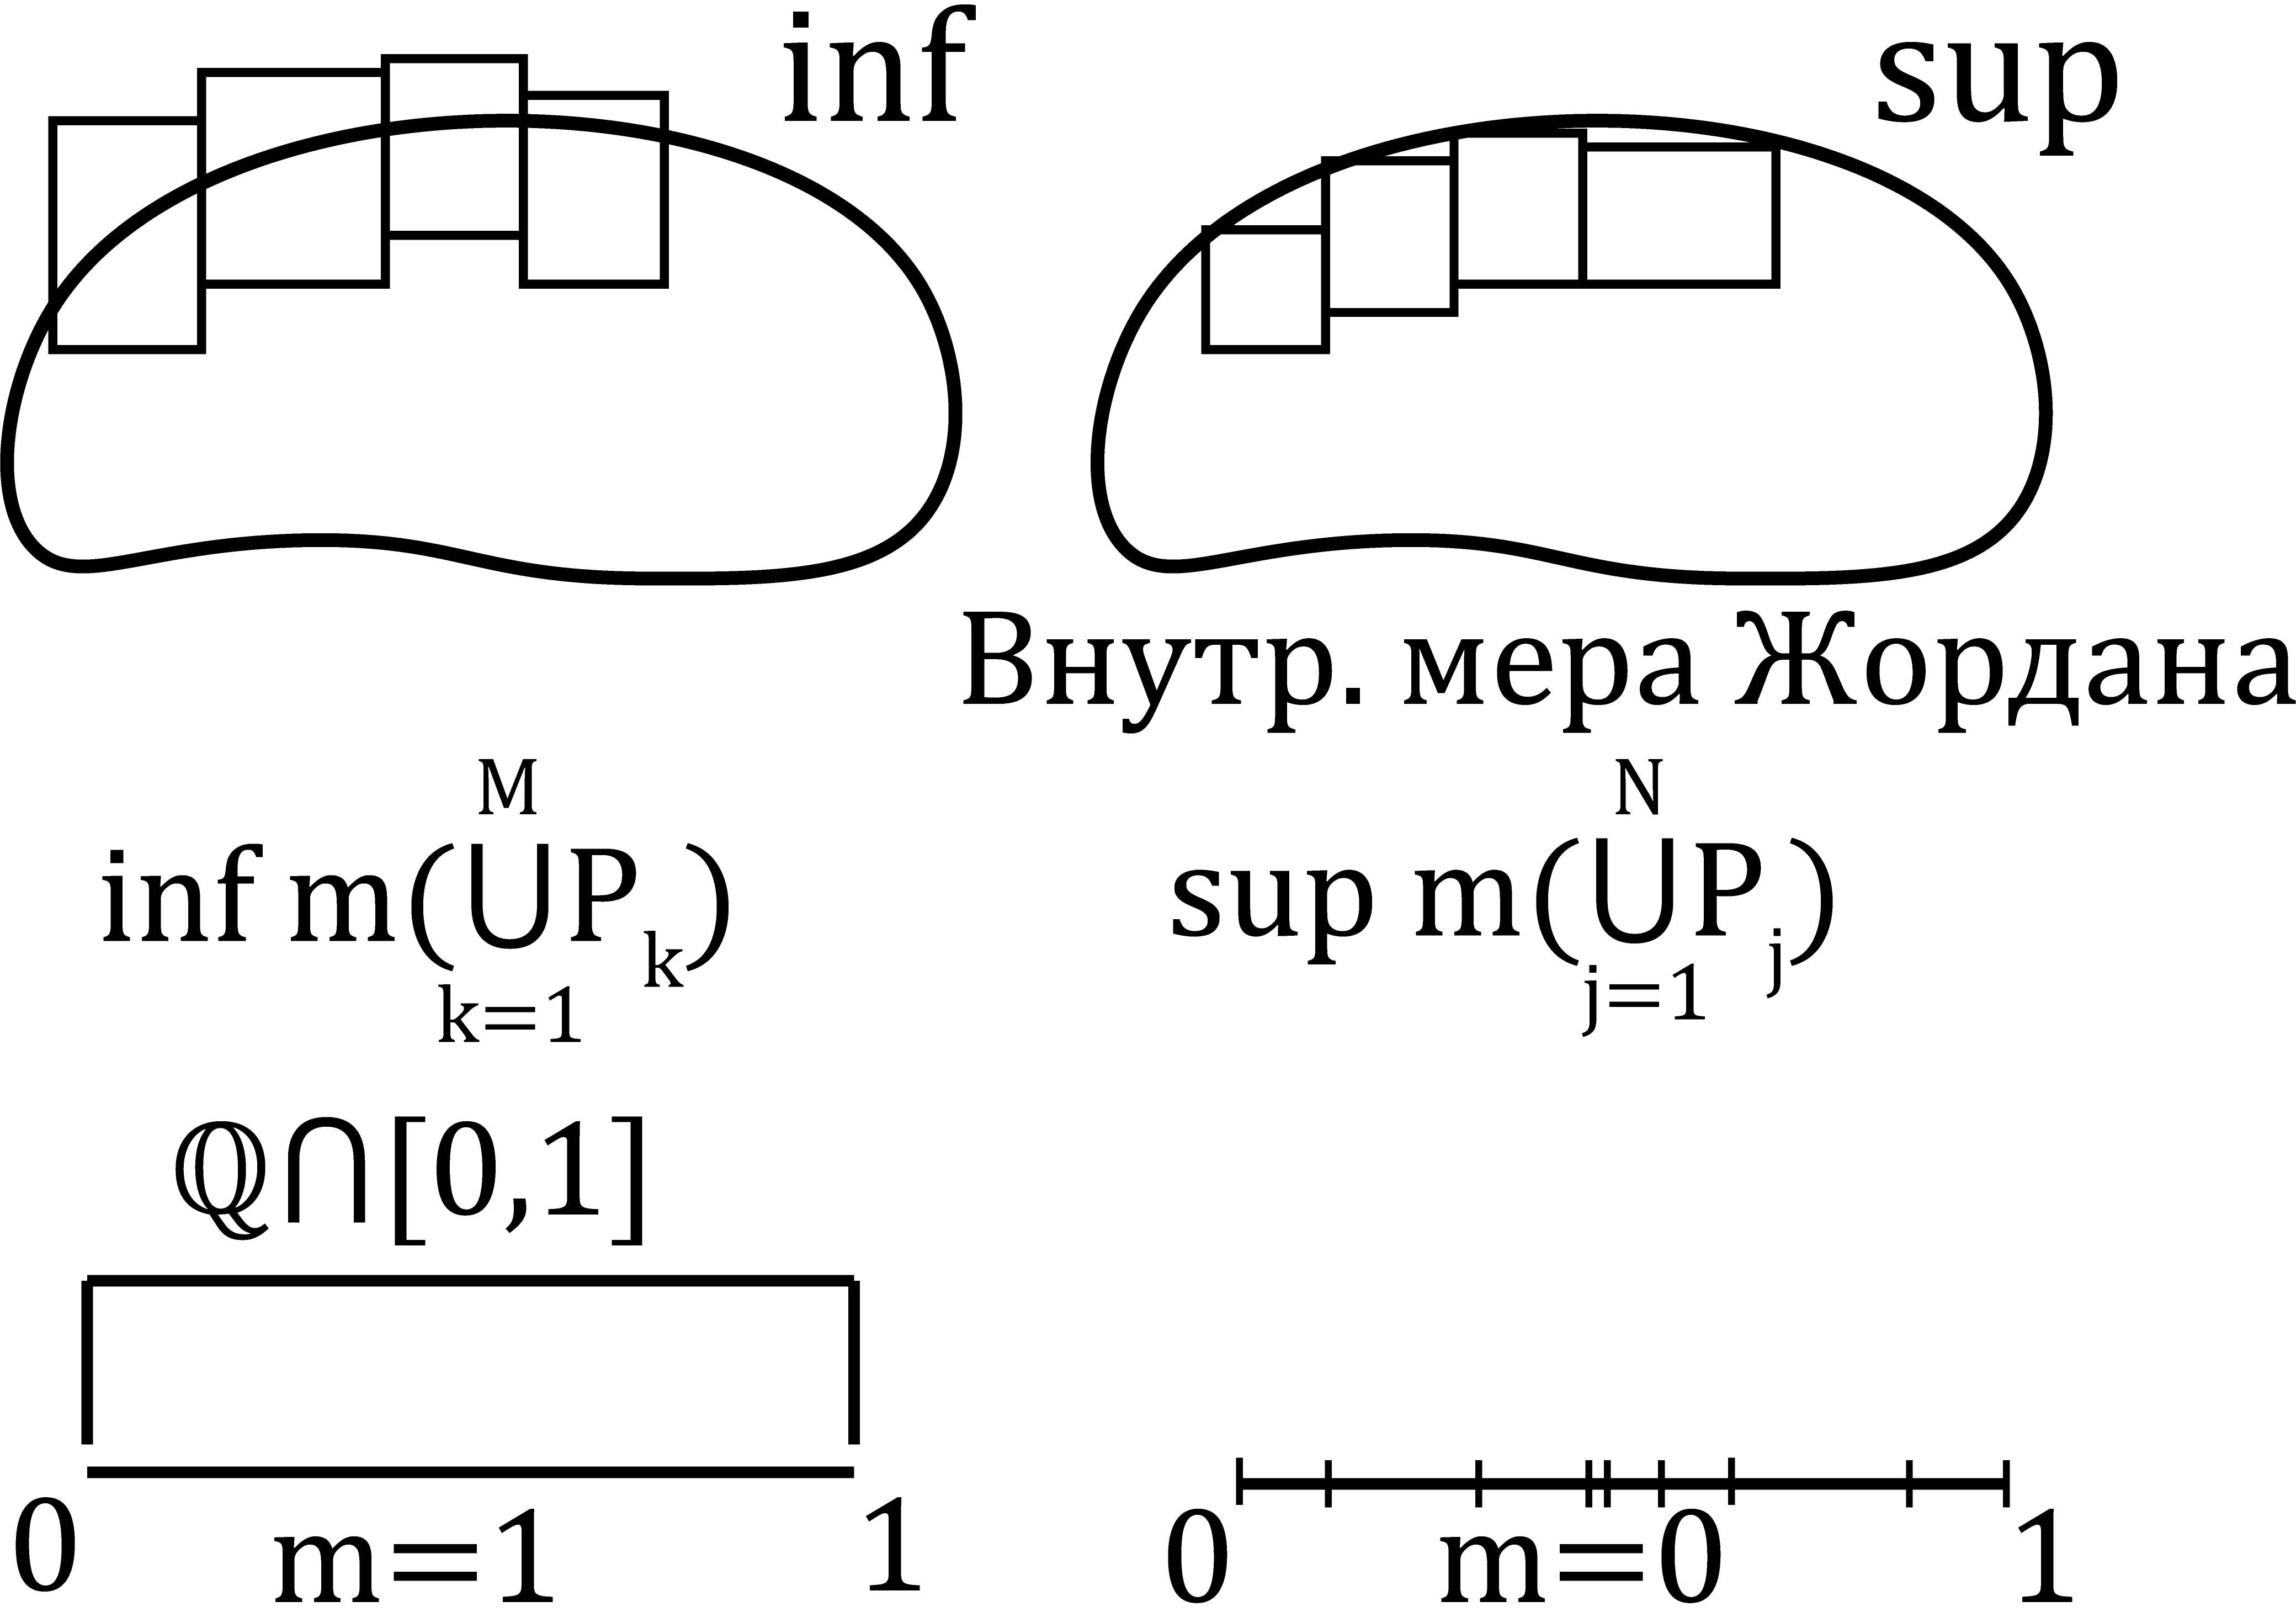
\includegraphics[width=6cm]{pics/14_10}
        \centering
    \end{figure}

    \begin{Definition}
        \[[0, 1]\]
        \[2^{[0, 1]} = \{A : A \subset [0, 1]\} \]
        \[\mathcal{A} \subset 2^{[0, 1]} \text{ --- нек. система подмножеств }[0, 1] \]
        \[\mu : \mathcal{A} \to [0, 1]\]
        \[\mu([a, b]) = b - a\]
        \[\mu(\varnothing) = 0\]
        \[A, B \in \mathcal{A} \q A \cap B = \varnothing \ \Ra \ \mu(A \cup B) = \mu(A) + \mu(B) \]
        \[A_1, ..., A_n, ... \in \mathcal{A} \Ra \bigcup_{k = 1}^\infty A_k \in \mathcal{A} \]
        \[\text{Если } A_j \cap A_k = \varnothing\]
        \[\Ra \mu(\bigcup_{k = 1}^\infty A_k ) = \sum_{k = 1}^\infty \mu (A_k) \]
        Инвариантность отн. пар. переноса\\
        %рисунок11
        \begin{figure}[H]
            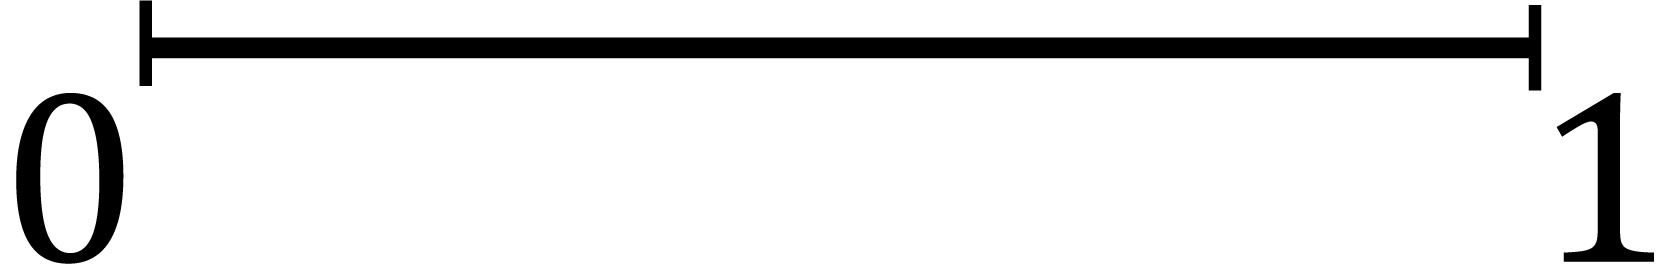
\includegraphics[width=3cm]{pics/14_11}
            \centering
        \end{figure}
        Отношение эквивалентности:
        \[x \sim y \ \rla \ x - y \in \Q\]
        В $\forall $ классе эквив-ти выберем представителя
        \[A = \{x \text{ - представитель кл. эквив., по одному из кажд. класса}\}\]
        \[\Q \text{ - счетное } \to  \text{ занумеруем его эл-ты}\]
        \[[0, 1] \cap \Q = \{\alpha_j\}_{i \in \N} \]
        \[A_j = \{a + \us{\in \Q}{\alpha_j},\  \forall a \in A\}\]
        \[A \cap A_j = \varnothing\]
        \[\forall j \neq k \q A_j \cap A_k = \varnothing\]
        \[[0, 1] = \bigcup_{j = 1}^\infty A_j; \q A_j \cap A_k = \varnothing \]
        \[\mu(A_j) = \mu(A_k) = \mu(A) \q(\text{т.к. получено пар. переносом})\]
        \[1 = \mu[0, 1] = \sum_{k = 1}^\infty \mu(A_k) \text{ --- ряд сх. } \ \Ra\  \mu(A) = 0?  \]
    \end{Definition}
\end{document}
